\section{The Eight Point Algorithm}

\paragraph{Introduction} We implemented the eight-point algorithm to estimate the fundamental matrix between two views of the same scene. The fundamental matrix $F$ is a $3 \times 3$ matrix that encapsulates the epipolar geometry between two images, allowing us to relate points in one image to epipolar lines in another. Our implementation follows the standard approach with the addition of point normalization for numerical stability and RANSAC for robust estimation.

\paragraph{Notation} In this section, we use the following notation:

\begin{itemize}
    \item $\mathbf{x}_i$, $\mathbf{x}'_i$: corresponding points in the first and second image, represented in homogeneous coordinates.
    \item $F$: the fundamental matrix.
    \item $l_i$, $l'_i$: epipolar lines in the first and second image corresponding to $\mathbf{x}'_i$ and $\mathbf{x}_i$.
\end{itemize}

\paragraph{Background} The fundamental matrix $F$ is a rank-2 matrix that satisfies the epipolar constraint for any pair of corresponding points $\mathbf{x}_i$ and $\mathbf{x}'_i$:

\begin{align*}
    {\mathbf{x}'_i}^T F \mathbf{x}_i = 0
\end{align*}

For a given point $\mathbf{x}_i$ in the first image, its corresponding epipolar line $l'_i$ in the second image can be computed as:

\begin{align*}
l'_i = F \mathbf{x}_i
\end{align*}

Similarly, for a point $\mathbf{x}'_i$ in the second image, its corresponding epipolar line $l_i$ in the first image is:

\begin{align*}
l_i = F^T \mathbf{x}'_i
\end{align*}

\paragraph{Methodology} Our implementation consists of several key components:

\begin{enumerate}
\item We obtained \textbf{point correspondences} between two images, either using manually annotated points or by automatically detecting and matching features using SIFT.
\item Before estimating the fundamental matrix, we \textbf{normalized} the coordinates by translating them so that their centroid is at the origin and scaling them so that the average distance from the origin is $\sqrt{2}$. This improves numerical stability.

\item Using at least 8 corresponding points, we set up a system of linear equations based on the epipolar constraint. Each correspondence provides one equation:

\begin{align*}
    x'_i x_i f_{11} + x'_i y_i f_{12} + x'_i f_{13} + y'_i x_i f_{21} + y'_i y_i f_{22} + y'_i f_{23} + x_i f_{31} + y_i f_{32} + f_{33} = 0
\end{align*}

Where $f_{ij}$ are the elements of $F$. We solve this system using Singular Value Decomposition (SVD).

\item Since $F$ must be of \textbf{rank 2}, we enforce this constraint by setting the smallest singular value to zero after SVD.

\item To handle potential outliers in the point correspondences, we implemented a RANSAC (Random Sample Consensus) approach. This involves:

\begin{itemize}
    \item Randomly sampling 8 correspondences
    \item Computing a candidate fundamental matrix
    \item Counting inliers (correspondences that satisfy the epipolar constraint within a threshold)
    \item Repeating the process multiple times and keeping the solution with the most inliers
\end{itemize}

\item We assessed the quality of our estimated fundamental matrix using the \textbf{geometric error}, which measures the average distance between points and their corresponding epipolar lines:

\begin{align*}
    \text{error} = \frac{1}{2n} \sum_{i=1}^{n} \left( d(\mathbf{x}_i, l_i) + d(\mathbf{x}'_i, l'_i) \right)
\end{align*}

where $d(\mathbf{x}, l)$ is the distance from point $\mathbf{x}$ to line $l$.
\end{enumerate}

\paragraph{Implementation} We implemented our solution in Python, using NumPy for matrix operations, OpenCV for image processing and feature detection, and Matplotlib for visualization. The config.json file allowed us to easily adjust parameters such as whether to use RANSAC, SIFT, or manual correspondences.

\begin{figure}[htbp]
    \begin{minipage}[t]{0.45\textwidth}
        \centering
        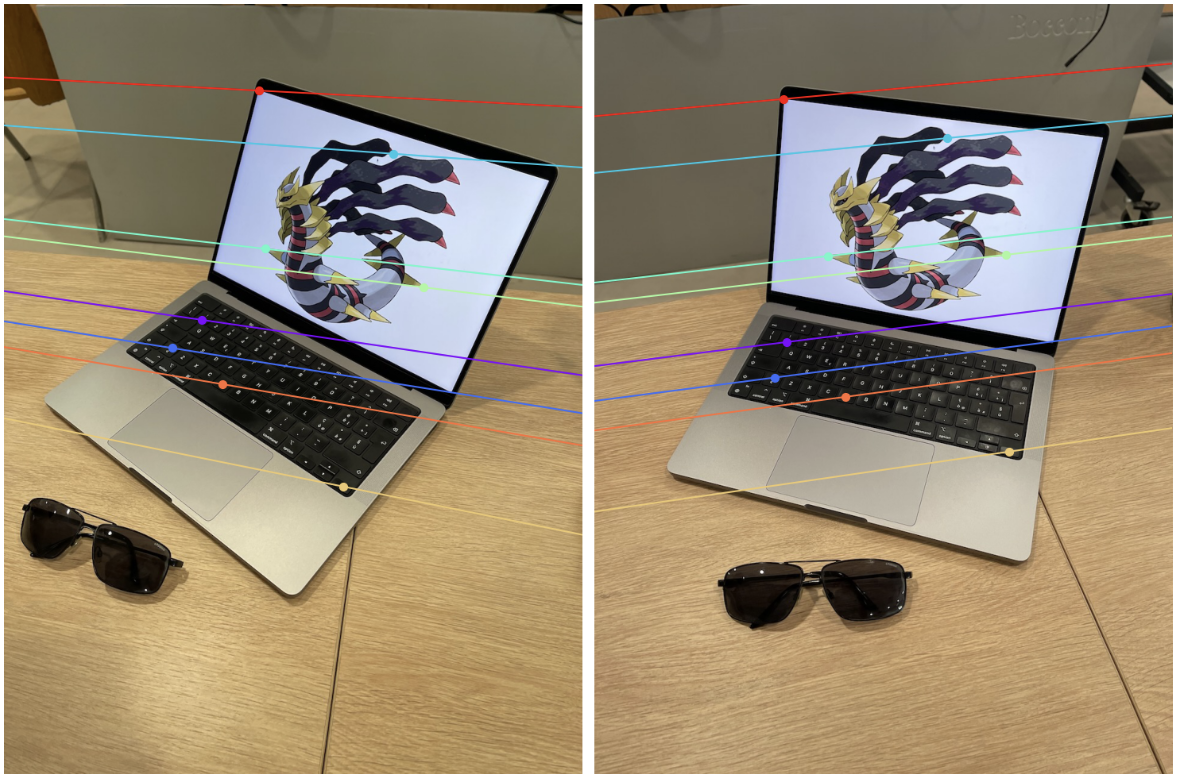
\includegraphics[width=\linewidth]{img/epipolar.png}
        \caption{Epipolar lines for the two views. Each point in one image corresponds to a line in the other image, and all these lines should intersect at the epipole (which is sometimes outside the visible image).}
        \label{epipolar}
    \end{minipage}
    \hfill
    \begin{minipage}[t]{0.45\textwidth}
        \centering
        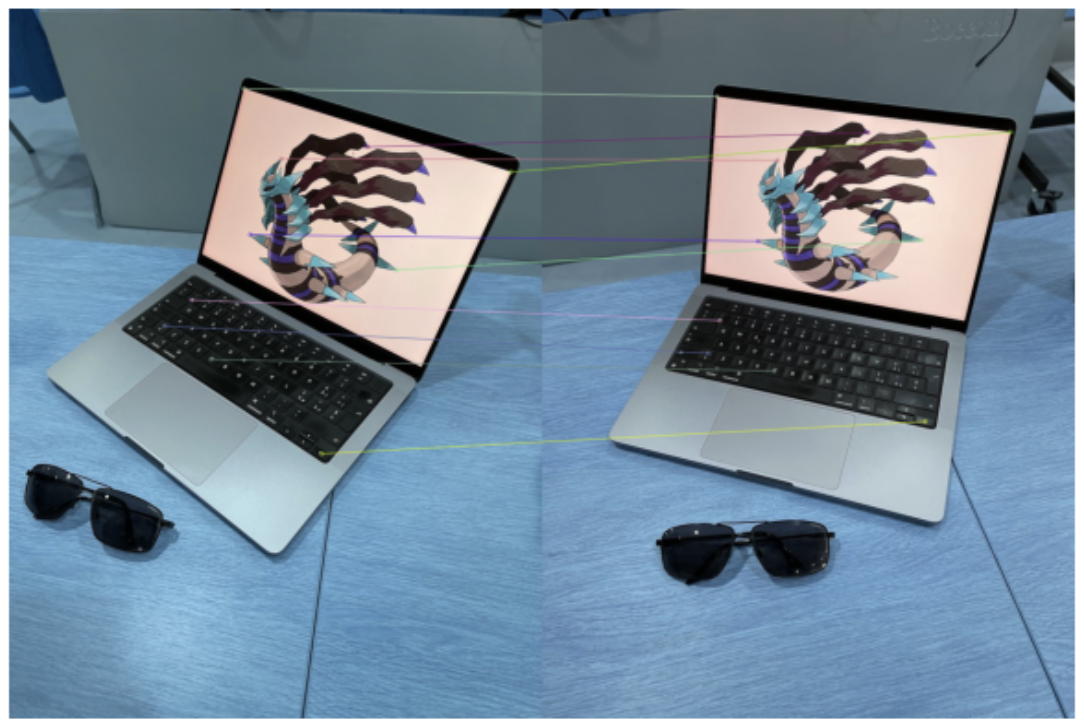
\includegraphics[width=\linewidth]{img/matches.png}
        \caption{Point correspondences between the two images. The lines connect matching points across the two views.}
        \label{matches}
    \end{minipage}
\end{figure}

\paragraph{Results} We tested our implementation on a pair of images taken from slightly different viewpoints (Figure \ref{matches}). Using RANSAC with 1000 iterations and an adaptive threshold, we achieved a mean geometric error of 0.64 pixels. The algorithm successfully identified 8 inliers out of 10 correspondences, resulting in an inlier ratio of 0.8.

\paragraph{Discussion} Our implementation of the eight-point algorithm with normalization and RANSAC proved effective in estimating the fundamental matrix and visualizing the epipolar geometry. We observed that normalization significantly improved the numerical stability of the algorithm, while RANSAC successfully handled outliers in the point correspondences.